\documentclass[letterpaper, 10pt, conference, twoside]{ieeeconf}


\IEEEoverridecommandlockouts
\overrideIEEEmargins
\usepackage{ctex}
\usepackage{booktabs}
\usepackage{graphicx}
\graphicspath{{figures/}}%图片所在的目录

\usepackage{lastpage}%获得总页数
\usepackage{fancyhdr}
\pagestyle{fancy}
%以下命令中L--左侧 R--右侧 C--中间 O--奇数页 E--偶数页
%\fancyhead[LO,RE]{机器学习原理、工程技术与应用}%奇数页左侧,偶数页右侧显示页眉
\fancyhead[CO,RE]{机器学习}%奇数页左侧,偶数页右侧显示页眉
\fancyhead[LO,CE]{代课教师 李乡儒,华南师范大学计算机学院}%奇数页左侧,偶数页中间页脚为空
\fancyhead[RO,LE]{\today}%奇数页右侧,偶数页左侧显示 当前页 of 总页数
\fancyfoot[CO,RE]{机器学习}%奇数页中间,偶数页右侧页脚为空
\fancyfoot[LO,CE]{2021-2022-2学期}%奇数页左侧,偶数页中间页脚为空
\fancyfoot[RO,LE]{\thepage\ of \pageref{LastPage}}%奇数页右侧,偶数页左侧显示 当前页 of 总页数
\renewcommand{\headrulewidth}{0.4pt}%改为0pt即可去掉页眉下面的横线
\renewcommand{\footrulewidth}{0.4pt}%改为0pt即可去掉页脚上面的横线
\setlength{\voffset}{-10mm}
\setlength{\topmargin}{0mm}
\setlength{\headheight}{5mm}
\setlength{\headsep}{5mm}
\setlength{\footskip}{8mm}



\title{\LARGE \bf
基于U-Net的混合注意力胃肠道图像分割
}


\author{2021023206 \quad 徐力\\ \today\\ 机器学习课程作业}

\usepackage{makecell}
\newcommand{\upcite}[1]{\textsuperscript{\textsuperscript{\cite{#1}}}}


\begin{document}

\maketitle
%\thispagestyle{empty}
%\pagestyle{empty}



\begin{abstract}
  分析了肠胃道图像分割竞赛数据的特点,包括掩码类别的占比、病例扫描次数分布、不同器官类别的共现性。通过观察掩码的重叠,制定了多标签分类的任务类型。分析了在扫描切片维度的掩码分布变化。提出了U-Net的三种改进方法以适用于竞赛数据集,即局部自注意力、外部注意力和邻居样本特征补全。设计了不同参数和下采样深度的两种U-Net变形结构,对比了两种结构的性能,并选择了结构较简单且泛化性能较优的4层U-Net结构。通过应用弹性畸变和高斯模糊,充实了训练数据,极大地提高了U-Net的泛化性能,改善了过拟合的问题。探究了几种损失函数,探究了其可用性,比较了不同损失函数的优缺点,通过实验确定了目前最佳比例的混合损失函数,并分析了平均准确率较低的可能的原因。提出了仍待解决的问题,给出了未来的改进思路。

\vspace{1ex}\noindent\textbf{关键词}: 医学图像分割;自注意力;U-Net;弹性畸变;损失函数

\end{abstract}


\section{引言}
医学图像分割是医学图像处理与分析领域的复杂而关键的步骤,其目的是将医学图像中具有某些特殊含义的部分分割出来,并提取相关特征,为临床诊疗和病理学研究提供可靠的依据,辅助医生作出更为准确的诊断。 医学图像具有复杂性,在分割过程中需要解决不均匀及个体差异等一系列问题,所以一般的图像分割方法难以直接应用于医学图像分割\cite{c1}。

UW-Madison 胃肠道图像分割(UW-Madison GI Tract Image Segmentation)是一场研究型代码竞赛\cite{c2},要求在医学扫描中跟踪健康肠胃器官的准确位置以改善肠胃癌的放射治疗。在治疗当中,借助集成磁共振成像和线性加速器系统(也称为 MR-Linacs)等技术,为了指向肿瘤施加高剂量辐射,同时避开肠和胃,放射肿瘤学家必须手动勾勒出胃和肠的位置。这项工作非常耗时,因为肿瘤、肠和胃的位置每天都在变化,使得治疗时间大大延长。

在比赛中,需要创建模型以在MRI扫描中自动分割肠和胃。在给出的数据集中,不同的患者在不同日子里进行了多次MRI扫描,每次扫描包括多张断层扫描。
% \subsection{二级标题}
% \subsubsection{三级标题}

\section{方法}
提出三种方法用于改进胃肠道MRI图像分割的精度,分别是局部自注意力、邻居样本特征补全和外部注意力。
\begin{table}[htbp]
  \centering
 \caption{多头局部自注意力算法}
 \label{tab:Algorithm1}
 \begin{tabular}{l}
  \toprule
  \textbf{算法一:多头局部自注意力} \\
  \midrule
    输入:X,形为(B,H,W,Win,C)的张量 \\
    其中,B是batch size;H,W为窗口所在的坐标;Win为窗口\\
    大小;C为feature map数量;Head为注意力头;HS为注意\\
    力头大小\\
    Q = query\_linear(X)  \# shape=(B,H,W,Win,C)\\
    K = key\_linear(X)\\
    V = value\_linear(X)\\
    \# shape=(B,H,W,Head,Win,HS)\\
    Q.resize();K.resize();V.resize() \\
    \# shape=(B,H,W,Head,Win,Win)\\
    attn\_sc = MatMul(Q,K.transpose(-1,-2))/sqrt(HS)\\
    attn\_sc = softmax(attn, dim=-1)\\
    \# shape=(B,H,W,Head,Win,HS)\\
    context = MatMul(attn\_sc,V)\\
    context.resize()  \# shape=(B,H,W,Win,C)\\
    attn\_out = linear(context)\\
    输出:attn\_out,形为(B,H,W,Win,C)的张量\\

  \bottomrule
 \end{tabular}
\end{table}
\subsection{局部自注意力}
自注意力模型\cite{attention}可用于捕捉输入序列的长程依赖关系,其引入了三个矩阵:键K、值V和查询Q矩阵。三个矩阵分别是对输入的线性变换。然而,Hongyi Wang\cite{MTM}等提出了一种适用于计算机视觉的局部注意力机制,仅关注每个固定大小的窗口内像素的相关性,仅在每个窗口内计算注意力系数而不是关注整个图像,从而减少计算开销的同时不影响性能。设定窗口大小为$Win = 4\times4=16$。归纳局部自注意力的实现方法如表1所示。

\subsection{邻居样本特征补全}
MRI扫描得到图片是灰阶的,为了输入U-Net模型,通常的做法是将单张灰阶图像广播到3个特征维上,以扩增张量维度。然而,单次MRI扫描得到的多张图片在特征上是连续变化的,即图片在位置上越相邻,相似度也越高,因此在直觉上,相邻的扫描切片可以提供相互映证的特征信息,以帮助判断一片区域像素的分类,即帮助提高图像分类的精度。而传统的方法将连续的扫描切片打散并输入U-Net模型,则丢失了这一连续性信息。

为了利用样本间连续性信息,提出的方法在预测单张扫描图片时,同时提供了与该图片相邻的前两张和后两张图片作为辅助分类信息。从而,模型的输入图像包含了5个通道,第3个通道是需要预测的图像,其余通道则是预测图像相邻的样本。

\subsection{外部注意力}
需要一种方法来建模邻居样本间,即输入的不同特征通道间的相关性。Meng-Hao Guo等\cite{EA}提出了称为外部注意力的方法,其在不同特征通道间通过softmax和L1正则化建立多头注意力。外部注意力可以考虑到不同样本间的潜在相关性。外部注意力的实现方法如表2所示。

\begin{table}[htbp]
  \centering
 \caption{外部注意力算法}
 \label{tab:Algorithm2}
 \begin{tabular}{l}
  \toprule
  \textbf{算法二:外部注意力} \\
  \midrule
    输入:X,形为(B,N,C)的张量 \\
    其中,B是batch size;N是图片像素数量;C为特征\\
    通道数量;Head为注意力头;HS为注意力头大小\\
    X = query\_linear(X)  \# shape=(B,N,4C)\\
    X.resize()  \# shape=(B,Head,N,HS)\\
    attn = linear0(X)  \# shape=(B,Head,N,2HS)\\
    \# shape=(B,Head,N,2HS)\\
    attn = softmax(attn, dim=-2)\\
    \# shape=(B,Head,N,2HS)\\
    attn = attn/sum(attn, dim=-1)\\
    X = linear1(attn)  \# shape=(B,Head,N,HS)\\
    X.resize()  \# shape=(B,N,4C)\\
    out\_X = project\_linear(X)  \# shape=(B,N,C)\\
    输出:out\_X\\
  \bottomrule
 \end{tabular}
\end{table}

\section{U-Net框架}
U-Net\cite{c3}的构建基于“全卷积网络”。它由收缩路径(左侧)和扩展路径(右侧)组成。收缩路径遵循卷积网络的典型架构。它由两个 3x3 卷积(未填充卷积)的重复应用组成,每个卷积后跟一个整流线性单元 (ReLU) 和一个 2x2 最大池化操作,步幅为 2,用于下采样。在每个下采样步骤中,我们将特征通道的数量加倍。扩展路径中的每一步都包括对特征图进行上采样,然后是将特征通道数量减半的 2x2 卷积(“上卷积”),与收缩路径中相应裁剪的特征图的连接,以及两个 3x3卷积,每个后跟一个 ReLU。由于在每个卷积中都会丢失边界像素,因此收缩路径中的图像需要经过裁剪,再与扩展路径中相应的图像拼接。在最后一层,使用 1x1 卷积将每个 64 分量特征向量映射到所需数量的类。该网络总共有 23 个卷积层,如图 1 所示。
\begin{figure}[htbp]
  \centering
  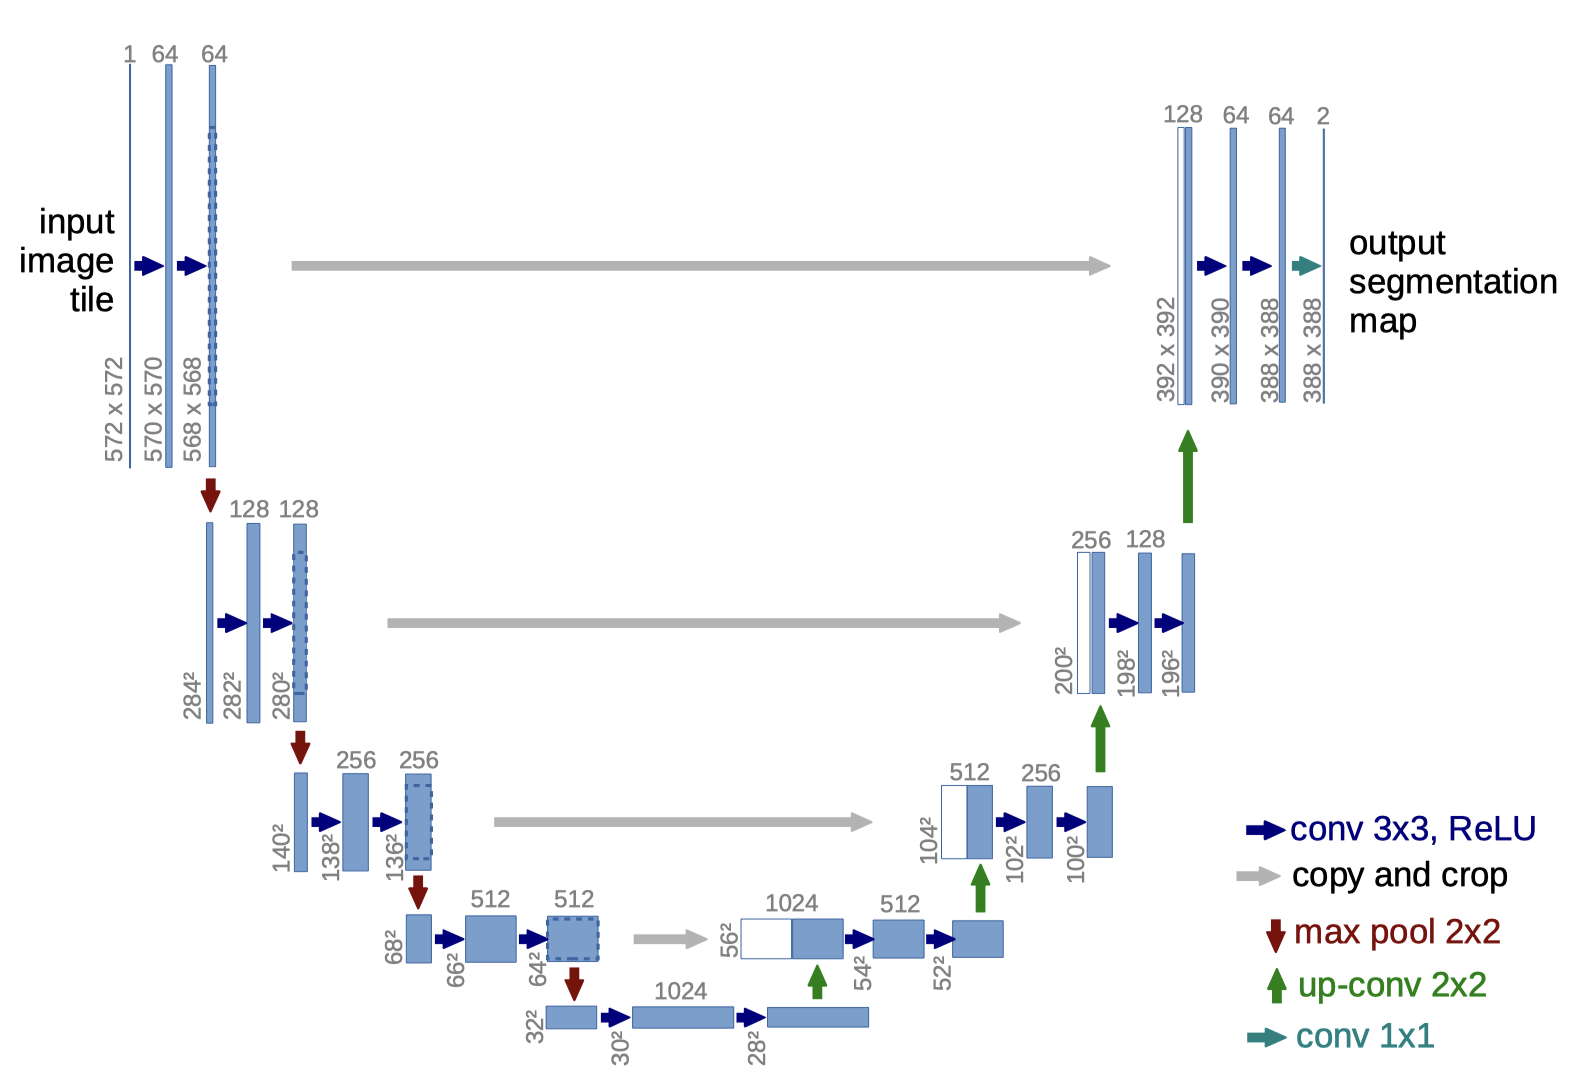
\includegraphics[width = 1\linewidth]{structure.png}
  \caption{U-Net 结构}
  \label{fig:fig1}
\end{figure}

在上采样部分,上采样的特征图包含了上下文信息,并与来自收缩路径的高分辨率特征结合,将上下文信息传播到更高分辨率的层。分割图只包含输入图像中完整上下文可用的像素,为了预测图像边界区域中的像素,通过镜像输入图像来推断缺失的上下文,如图2所示。

\begin{figure}[htbp]
  \centering
  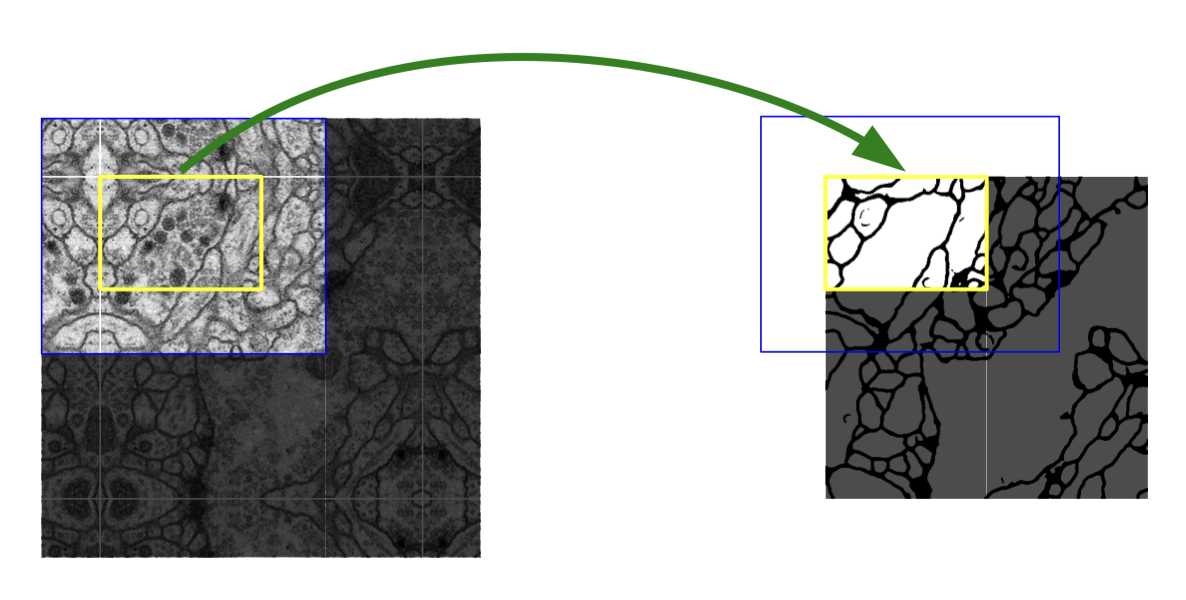
\includegraphics[width = 1\linewidth]{seamless-seg.png}
  \caption{镜像拼接原图,以补充边缘像素缺失的上下文}
  \label{fig:fig2}
\end{figure}

生物医学图像分割中,可用的训练数据通常较少。因此,需要对可用的训练图像应用数据增强,如弹性变形等。这允许网络学习对此类变形的不变性。同时在生物医学当中,变形曾经是组织中最常见的变化,并且可以有效地模拟真实的变形。通过数据增强,模型学习数据的不变性特征,从而防止过拟合。


\section{赛题数据分析}

竞赛给出16位灰度 PNG 图像,参赛者需要在图像中分割器官细胞。训练注释以 RLE 编码掩码的形式提供。

比赛中有多个病例,每个病例的扫描分为多组,每组由扫描发生的日期标识,扫描的当天产生多张扫描切片。一部分病例按照扫描日期的先后划分为训练集和测试集;另外一部分病例的全部数据处于训练集或测试集中。因此,模型不仅需要针对见过的病例标注其器官位置,也需要标注完全没见过的病例。

训练集中,每个病例的扫描次数(天数)在1到6之间。

\begin{table}[htbp]
  \centering
 \caption{数据集的统计数据}
 \label{tab:table1}
 \begin{tabular}{llll}
  \toprule
  \makecell[l]{注释数量\\(图片数量)} & 病例数量 & \makecell[l]{无掩码\\图片数量}& \makecell[l]{有掩码\\图片数量}\\
  \midrule
    38496&85&21906&16590\\
  \bottomrule
 \end{tabular}
\end{table}

\begin{table}[htbp]
  \centering
 \caption{扫描次数统计}
 \label{tab:table2}
 \begin{tabular}{l|ccccccc}
  \toprule
  \makecell[l]{扫描\\次数}& 1次 & 2次 & 3次 & 4次 & 5次 & 6次 & 合计\\
  \midrule
  \makecell[l]{病例\\数量}& 9 & 8 & 45 & 2 & 20 & 1 & 85\\
  \bottomrule
 \end{tabular}
\end{table}

\begin{table}[htbp]
  \centering
  \caption{胃、大肠和小肠的共现;其中对角线上的数字表示该器官的总出现次数}
  \label{tab:table3}
\begin{tabular}{||c||c|c|c||}
\hline
次数&胃&大肠&小肠 \\
\hline\hline
胃&8627&6181&3361 \\
\hline
大肠&6181&14085&10982 \\
\hline
小肠&3361&10982&11201 \\
\hline
\end{tabular}
\end{table}


\begin{figure}[htbp]
  \centering
  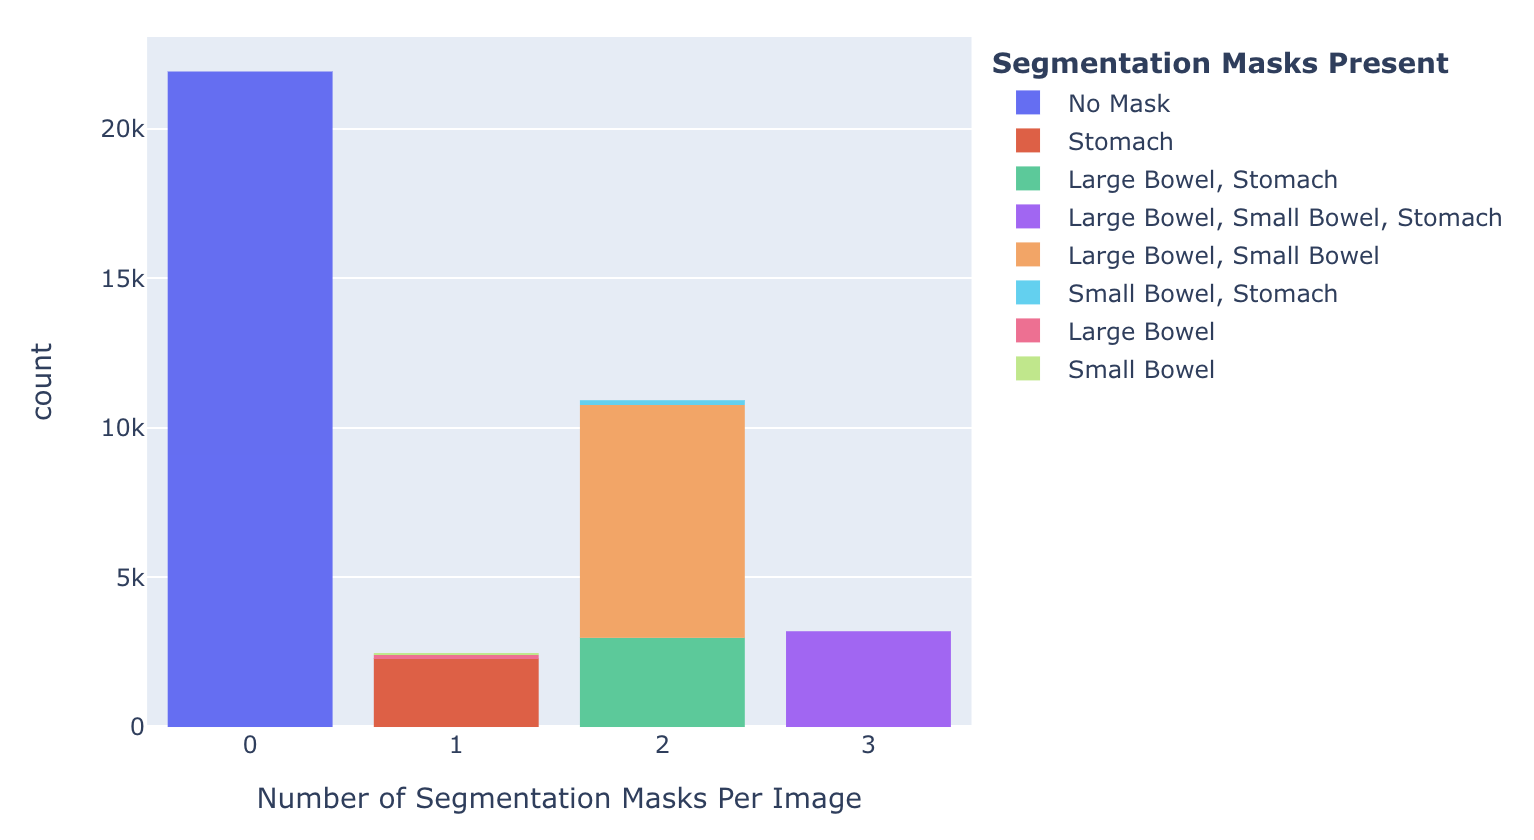
\includegraphics[width = 1\linewidth]{nseg-per-img.png}
  \caption{每张图片的分割掩码数量}
  \label{fig:fig3}
\end{figure}

如表1所示,数据集中一共有38496张图片,其中没有掩码的图片有21906张,占56.9046\%;有至少一类掩码的图片有16590张,占43.0954\%。这些扫描图片来自一共85个病例。

每个病例的扫描次数(天数)在1次(天)到6次(天)之间,如表2所示。其中,最多的病例(45例)是扫描了3次,其次(20例)是扫描了5次。按照比赛规则,部分病例的不同阶段的扫描被分别划分到了训练集和测试集,这可能是扫描次数分布不规律的原因。

进一步统计当图片的掩码分别存在0、1、2、3类时对应的各器官种类的数量,如图3所示。没有注释的情况可在表1中观察,下面分别观察图片存在1、2、3种掩码的情况:

\subsection{存在一种掩码的图片}
存在且仅存在一种掩码的图片一共有2468张,占6.41\%。在这些注释当中,大多数的注释是关于胃。其中,胃的注释有2286个,占92.6\%;大肠的注释有123个,占4.98\%;小肠的注释有59个,仅占2.39\%。

\subsection{存在两种掩码的图片}
存在且仅存在两种掩码的图片一共有10921张,占28.37\%.在这些注释当中,大多数的注释的组合是关于大肠和小肠。其中,大肠-小肠的注释有7781个,占71.3\%;大肠-胃的注释有2980个,占27.3\%;小肠-胃的注释有160个,仅占1.47\%。

\subsection{存在三种掩码的图片}
存在三种掩码的图片一共有3201张,占8.32\%.

如表3所示。所有注释一共有33913条,其中最多的种类是大肠(14085条),其次是小肠(11201条)、胃(8627条),分别占41.53\%,33.03\%,25.44\%.一次共现在这里表示为一对注释在同一张扫描图片上同时出现。胃-大肠、大肠-小肠、小肠-胃的共现分别是6181、10982、3361。可见,断层扫描图片中,最常同时出现器官的是大肠和小肠,最少同时出现的是小肠和胃。造成的原因可能是身体结构导致的器官分布规律:大肠通常分布在胃的下方,而小肠分布在大肠的下方。

数据集中的图片尺寸主要有(266,266)和(310,360)两种,此外还有(276,276)和(234,234),如表4所示。

\begin{table}[htbp]
  \centering
  \caption{不同尺寸的图片数量}
  \label{tab:table4}
  \begin{tabular}{cccc|c}
    \toprule
    (266,266)&(310,360)&(276,276)&(234,234)&合计 \\
    \midrule
      25920&11232&1200&144&38496\\
    \bottomrule
   \end{tabular}
\end{table}

数据集注释采用游程编码(RLE, run-length encoding)格式。每个像素可以属于背景,或大肠、小肠、胃当中的一类或多类。典型掩码标签的可视化如图4所示。部分器官分割注释是有重叠的,如图5所示,有一部分大肠的注释完全处于小肠的注释当中。因此本竞赛是逐个像素的多标签多分类任务。

\begin{figure}[htbp]
  \centering
  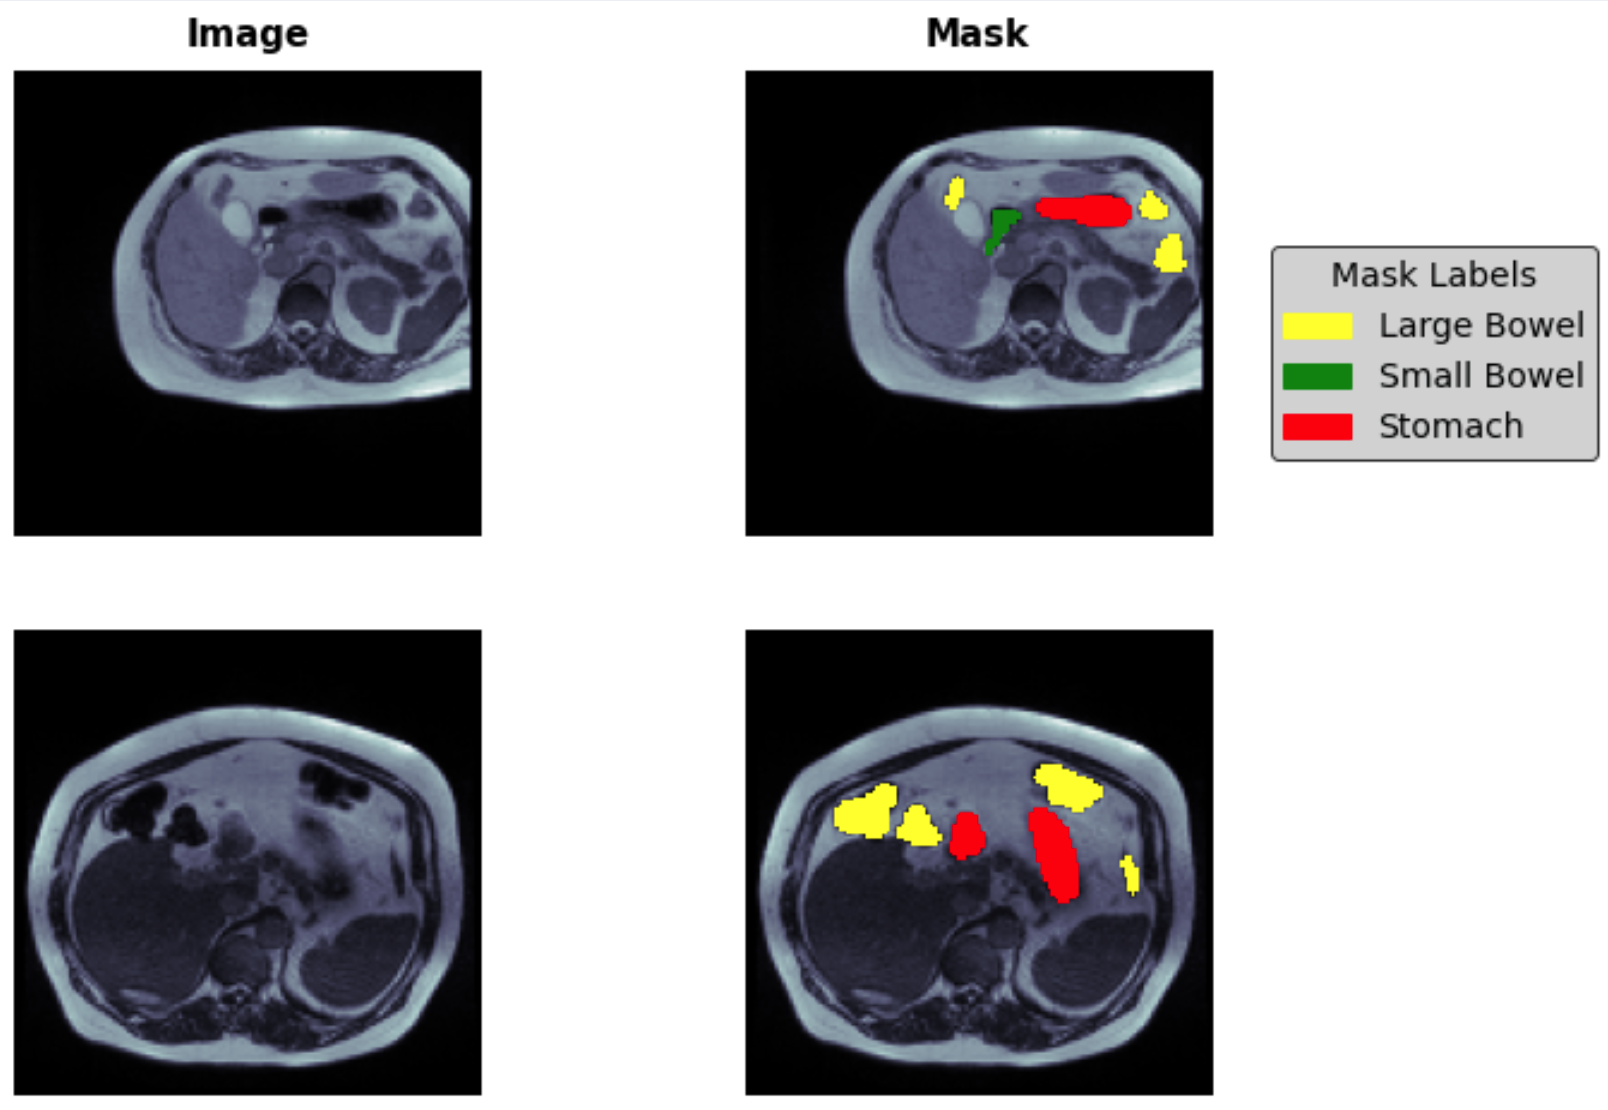
\includegraphics[width = 1\linewidth]{seg_view.png}
  \caption{典型的掩码标签注释}
  \label{fig:fig4}
\end{figure}

\begin{figure}[htbp]
  \centering
  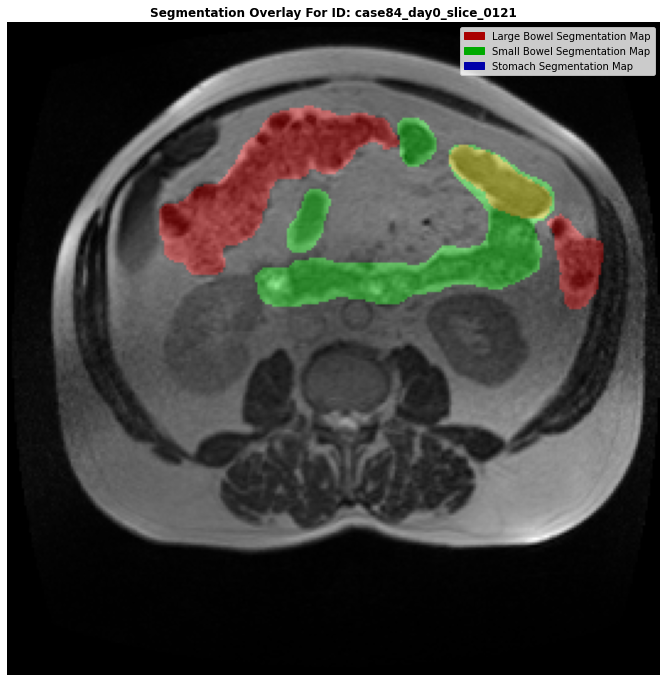
\includegraphics[width = 1\linewidth]{seg_overlay.png}
  \caption{重叠的掩码标签注释}
  \label{fig:fig5}
\end{figure}

为了进一步探究将竞赛作为单标签多分类处理会造成的损失,统计不同种类和不同大小的掩码重叠发生的次数,如图12所示。胃-大肠-小肠重叠掩码的面积可达到300以上;大肠-小肠重叠掩码的面积可达到600以上。因此,掩码应表示为$W\times H\times 3$。其中3个通道分别表示不同的掩码类型。

对于给定的病例和扫描天数为单次扫描。单次扫描得到一系列连续的断层切片,得到的切片数量有两种情况:144张或80张。一共259次扫描是144张,15次扫描是80张。统计所有不同位置的切片包含器官掩码的数量,分布近似钟形曲线,如图6所示。观察得到,胃、大肠、小肠在扫描切片上分布达到峰值所在的位置分别为67、100、102,对应的最大注释数量分别为196、240、235个。大肠和小肠对峰值以左的切片位置有所偏置,而胃有向右的偏置。小肠、胃的扫描切片位置相对大肠较为集中。可见,器官扫描切片数量峰值的位置排序符合器官的大致高低位置排序(胃>大肠>小肠);而峰值的注释数量排序符合各器官总注释数量的排序(大肠>小肠>胃)。

\begin{figure}[htbp]
  \centering
  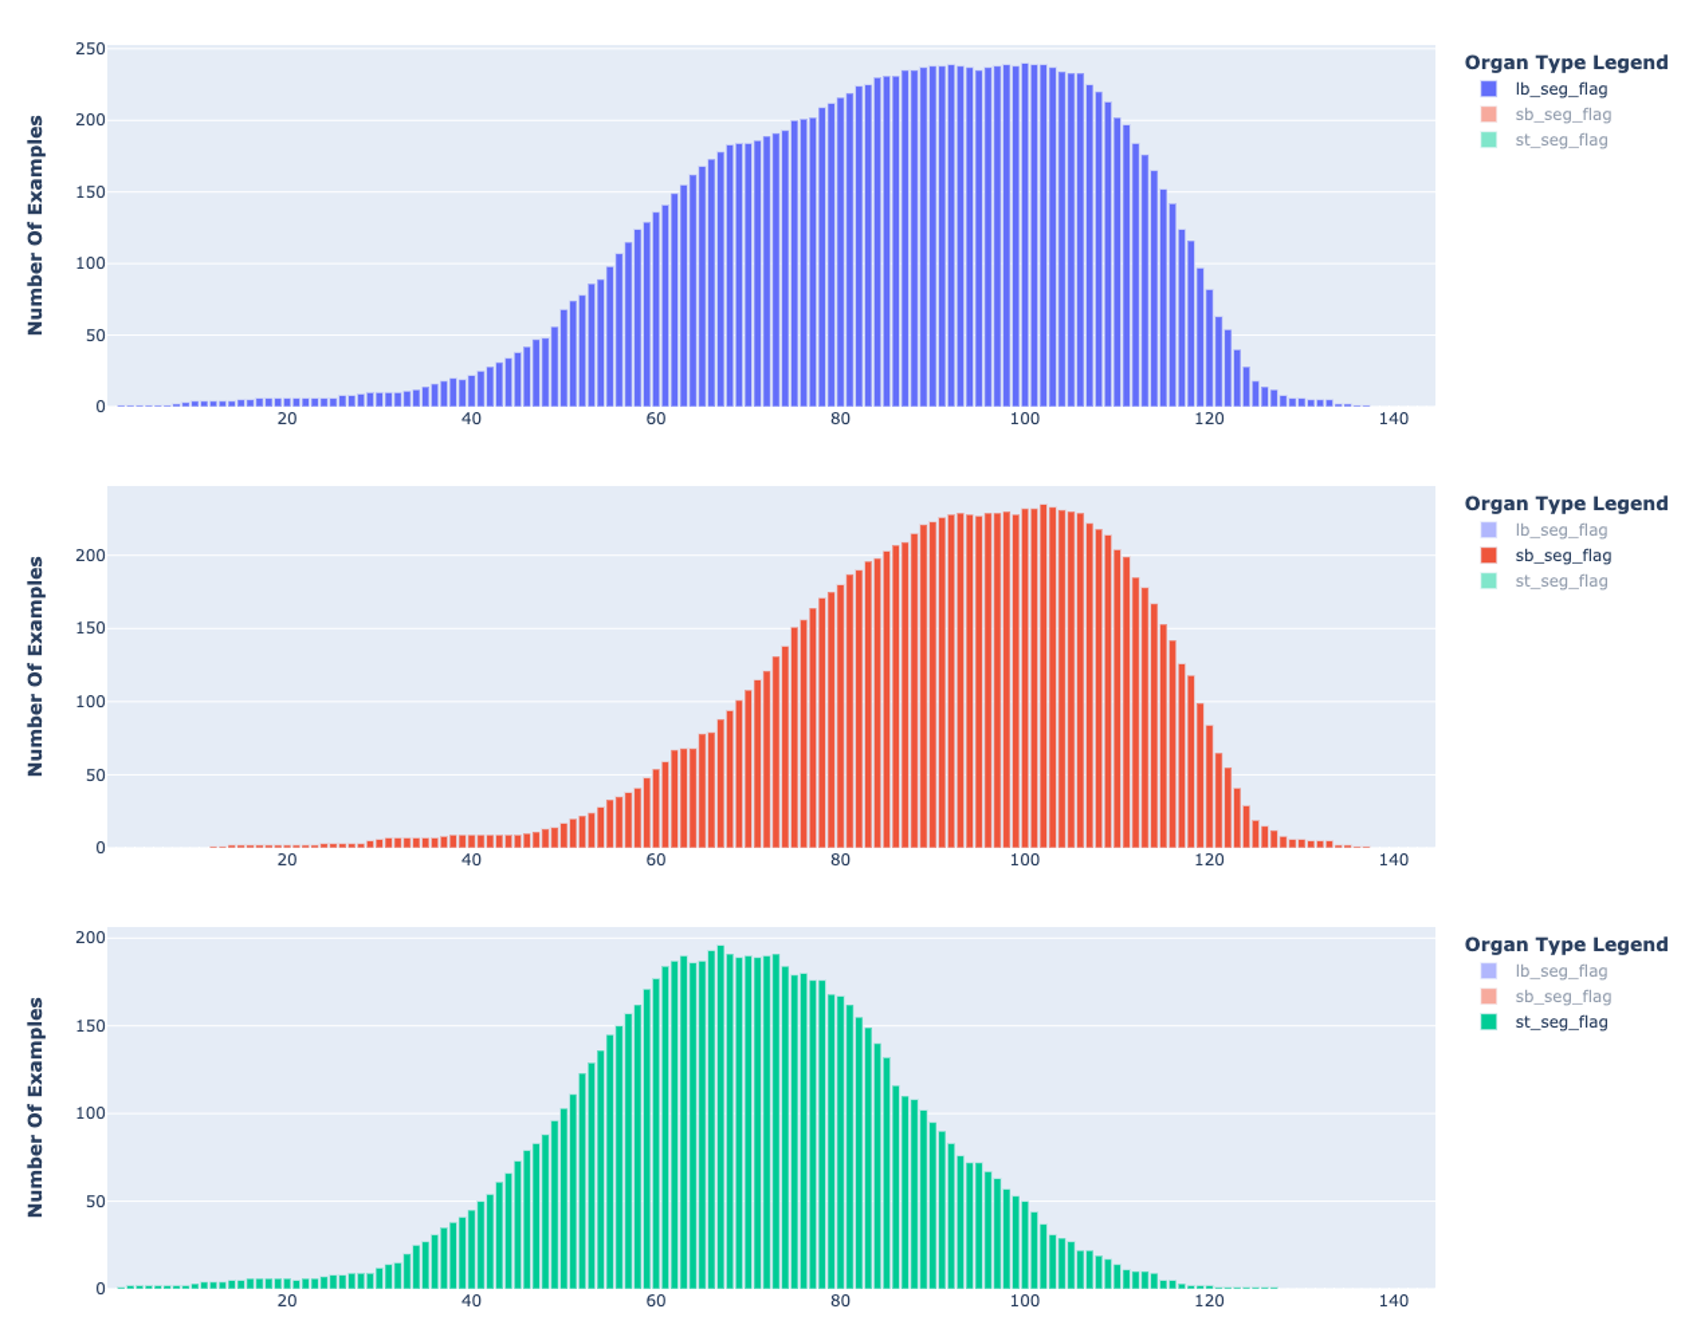
\includegraphics[width = 1\linewidth]{seg_distribution.png}
  \caption{分割掩码重叠面积的分布}
  \label{fig:fig6}
\end{figure}

\section{实验}
\subsection{评价指标}

竞赛根据平均骰子系数(Dice coefficient)和3D豪斯多夫距离(Hausdorff distance)评估结果。

平均骰子系数是每张图片的Dice系数的平均值:
\[SC_{Dice}\]

3D豪斯多夫距离(Hausdorff distance)的计算:首先使用扫描切片构建3D图像,每个切片的深度为1,计算预测物体到基准物体的豪斯多夫距离并归一化,取每张图片的平均,最后转化为分数:
\[ SC_{Haus} \]

最终分数是两个分数的加权和,计算如下:
\[SC_{Final} = 0.4 * SC_{Dice} + 0.6 * SC_{Haus}\]

\subsubsection{骰子系数}

设$X$是预测像素的集合,$Y$是基准像素的集合,则Dice系数计算如下:

\[ \frac{2*|X\cap Y|}{|X|+|Y|}\]

Dice系数用于度量两个集合之间的一致性。当 X 和 Y 都为空时,Dice 系数定义为 0。

\subsubsection{豪斯多夫距离}

竞赛中的豪斯多夫距离指的是有向豪斯多夫距离,即一个点集中的点到另一个点集中的点的最短距离的最大值。设$X$是预测物体像素的集合,$Y$是基准物体像素的集合,则3D豪斯多夫距离计算如下:
\[\sup_{x\in X} \inf_{y\in Y} d(x,y)\]
其中sup和inf分别表示上确界和下确界。

\subsection{实验设置}

\subsubsection{训练集划分}

实验采用5折交叉验证,需要将样本随机分成数量大致相等的五个数据集。划分的过程还需要满足一些要求:第一,每个病例作为一个组,且每个组中的所有数据必须处于同一折当中。否则,若一个病例的部分数据处于训练集且另一部分处于验证集,则会出现数据泄漏的问题。第二,每折数据应包含所有的分类,即背景、胃、大肠和小肠,且每折数据包含的各类别应尽量保持等比例,以防止数据不平衡的问题。

使用keras中的StratifiedGroupKFold方法,将图片中分别有0、1、2、3个类别作为标签,并按病例分组,即可划分5折交叉验证数据集并满足以上两点要求。

\subsubsection{模型结构}

对U-Net进行修改以适应数据集:
第一,U-Net原输入张量为$572\times 572\times 1$,为了适应肠胃的多标签分类,输入张量修改为$128\times 128\times 3$,每个通道表示一个类别的掩码。

第二,每个$3\times 3$卷积包含padding操作,不改变图像尺寸,从而保持了收缩路径和扩展路径尺寸的一一对应,在拼接操作时,高分辨率图像不需要裁剪,从而保留了高分辨率图像的边缘信息。在unet++等文献中,同样是这种做法。

第三,比较了两种结构:收缩路径下采样深度为4或5,最深层神经元的感受野分别为125和253,而图像的输入大小为128$\times$128,略大于4层unet的最大下采样感受野,小于5层unet的最大下采样感受野,如表5所示。

\begin{table}[htbp]
  \centering
  \caption{4层和5层unet的每层下采样前的理论感受野}
  \label{tab:table5}
  \begin{tabular}{ccc||ccc}
    \toprule
    \multicolumn{3}{c}{\textbf{4层下采样}} & \multicolumn{3}{c}{\textbf{5层下采样}} \\
    \toprule
    层&输入大小&感受野&层&输入大小&感受野 \\
    \midrule
      0&128&5$\times$5&0&128&5$\times$5 \\
    \midrule
      1&64&13$\times$13&1&64&13$\times$13 \\
    \midrule
      2&32&29$\times$29&2&32&29$\times$29 \\
    \midrule
      3&16&61$\times$61&3&16&61$\times$61 \\
    \midrule
      4&8&125$\times$125&4&8&125$\times$125 \\
    \midrule
      /&/&/&5&4&253$\times$253 \\
    \bottomrule
   \end{tabular}
\end{table}



\subsubsection{训练设置}

以二元交叉熵损失函数作为优化目标,使用Adam算法作为优化器。度量函数为骰子系数、交并比系数和准确率。实验在i5-8400 CPU和RTX3080 GPU的Linux服务器上进行。

\subsection{初步实验结果分析}

\begin{figure}[htbp]
  \centering
  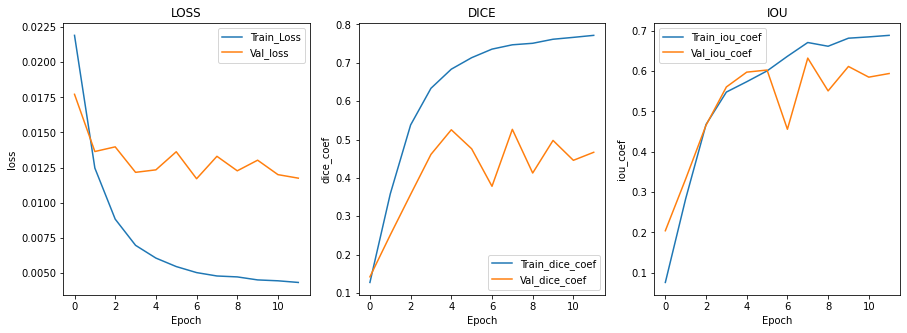
\includegraphics[width = 1\linewidth]{metric_result.png}
  \caption{损失函数和度量函数的优化过程}
  \label{fig:fig7}
\end{figure}

如图7所示,初步的实验取得了50\%以上的验证集上Dice系数。由于设置了早停,在连续5轮的验证集损失没有低于第6轮的损失之后,训练停止。由此可见,过拟合是亟待解决的问题。

模型预测的可视化如图9所示。可以观察到,对于已经判断正确的器官,模型预测的边界倾向于收缩,即将一些器官的边缘像素分类为背景。同时,模型可能将背景误分类为器官。

\subsection{数据增强}

为了解决模型的过拟合的问题,对训练集进行数据增强。弹性畸变\cite{c5}是一种适用于生物细胞组织的数据增强方法,这有利于模型学习在这种畸变当中的不变性,而畸变是器官组织很常见的变化。同时加入高斯噪声从而突出图像的低频特征。数据增强的效果如图8所示。

\begin{figure}[htbp]
  \centering
  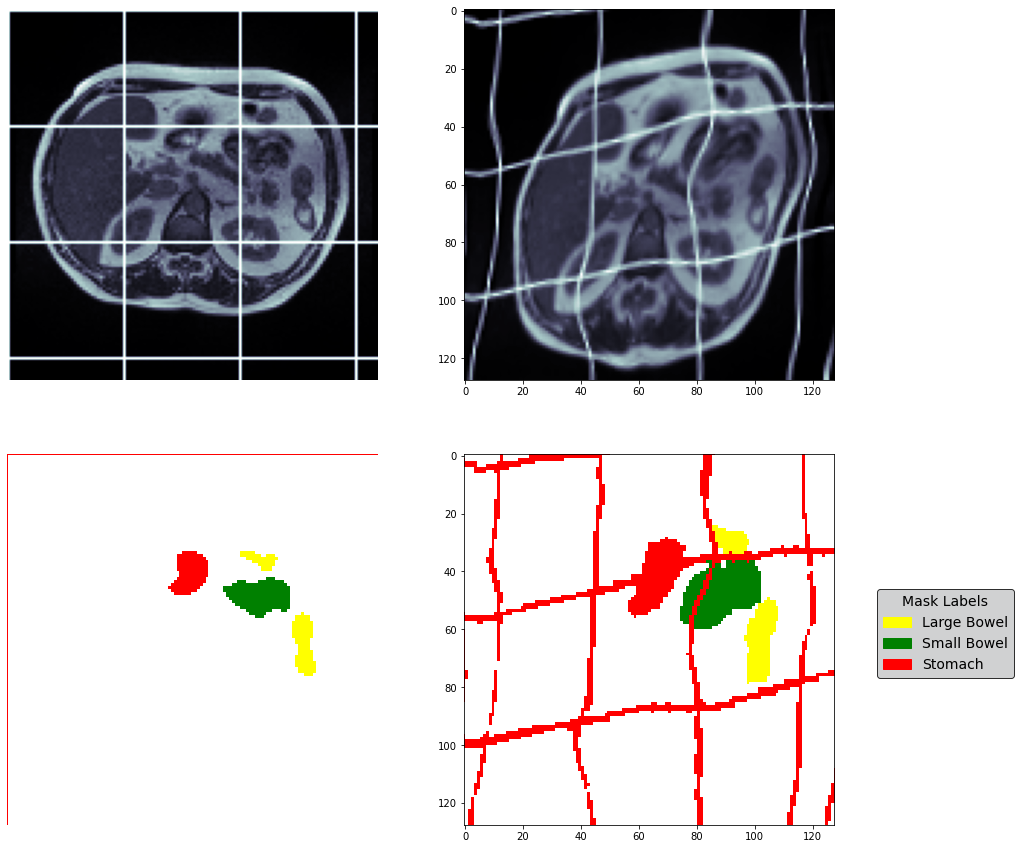
\includegraphics[width = 1\linewidth]{elastic3.png}
  \caption{数据增强效果;左上:原图(加入栅格以更明显地查看畸变程度);右上:加入数据增强的图像;左下:大肠、小肠和胃的掩码图像;右下:加入数据增强的掩码图像}
  \label{fig:fig8}
\end{figure}

数据增强后的损失函数、Dice系数和IOU系数的优化过程如图9所示。验证集上损失在第19轮达到极小值,并直到第34轮没有明显的降低或提升,因此在34轮进入早停。可见,在20轮训练之前没有出现过明显的拟合问题。此外,与未经过数据增强相比较,最优Dice系数也从0.5提升到0.7006,最优交并比则从0.6提升到0.7699.并且,训练集的交并比也有所提升。

\begin{figure}[htbp]
  \centering
  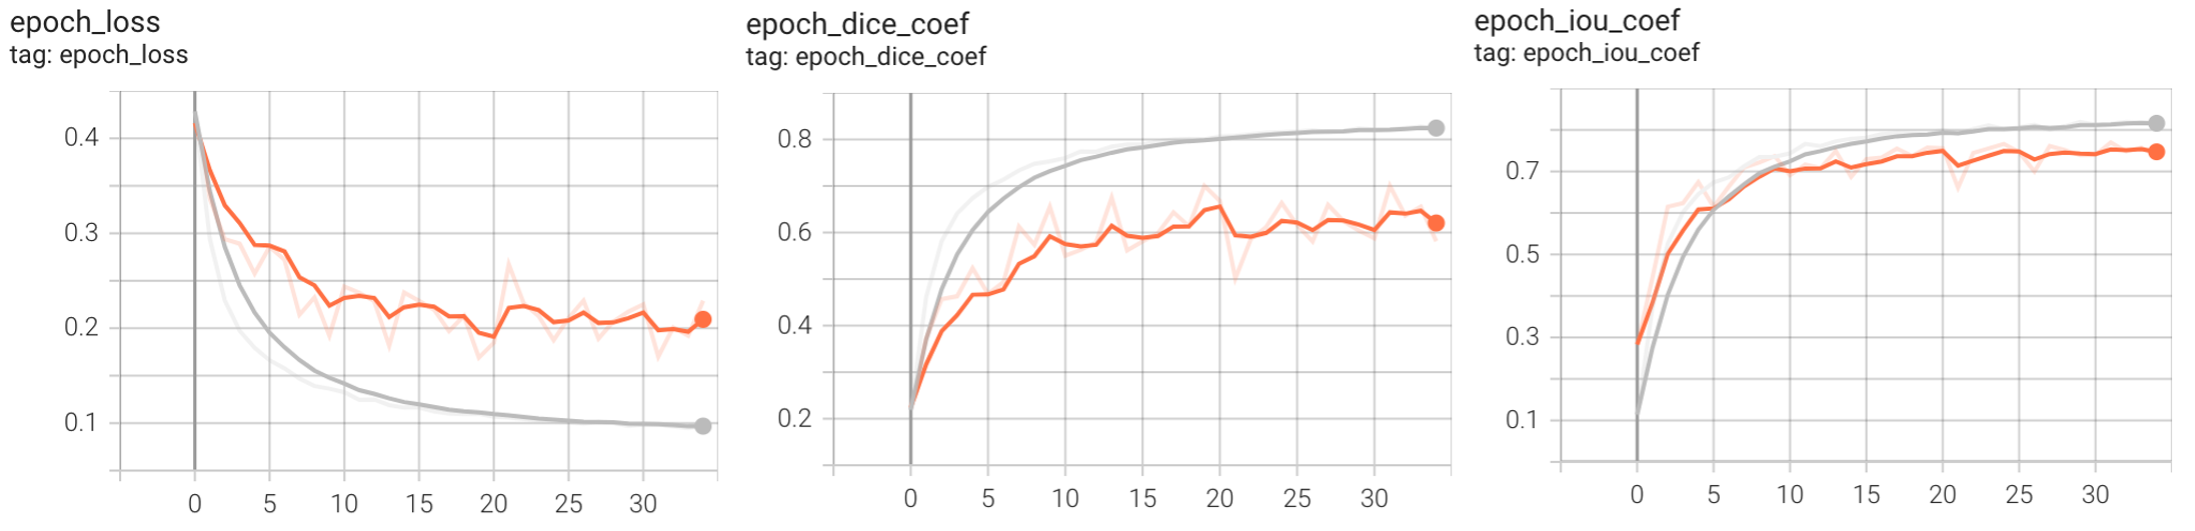
\includegraphics[width = 1\linewidth]{dataAug_result.png}
  \caption{数据增强后的损失函数、Dice、IOU优化过程(曲线有60\%的平滑)}
  \label{fig:fig9}
\end{figure}

\subsection{4层unet和5层unet的比较}

为了探究增加下采样层数是否会提升模型的性能,分别构建了4层unet和5层unet,采取相同的数据增强方法和学习率等超参数,并对比它们的性能。4层unet和5层unet的参数数量分别为2.50兆和5.72兆。训练结果如图10所示。

可见,4层和5层unet的loss、Dice系数、IOU无明显差异,验证集上最优Dice系数均处在0.7附近,验证集上最优交并比均在0.75附近。然而,在15轮等待的早停中,4层unet的最优损失出现在第27轮且训练了39轮(最大训练轮数为40轮);而5层unet的最优损失出现在第19轮且训练了34轮。因此可以认为,参数更少的4层unet的泛化性能优于参数更多的5层unet,而5层unet并没有学习到比4层unet更多的特征。

\begin{figure}[htbp]
  \centering
  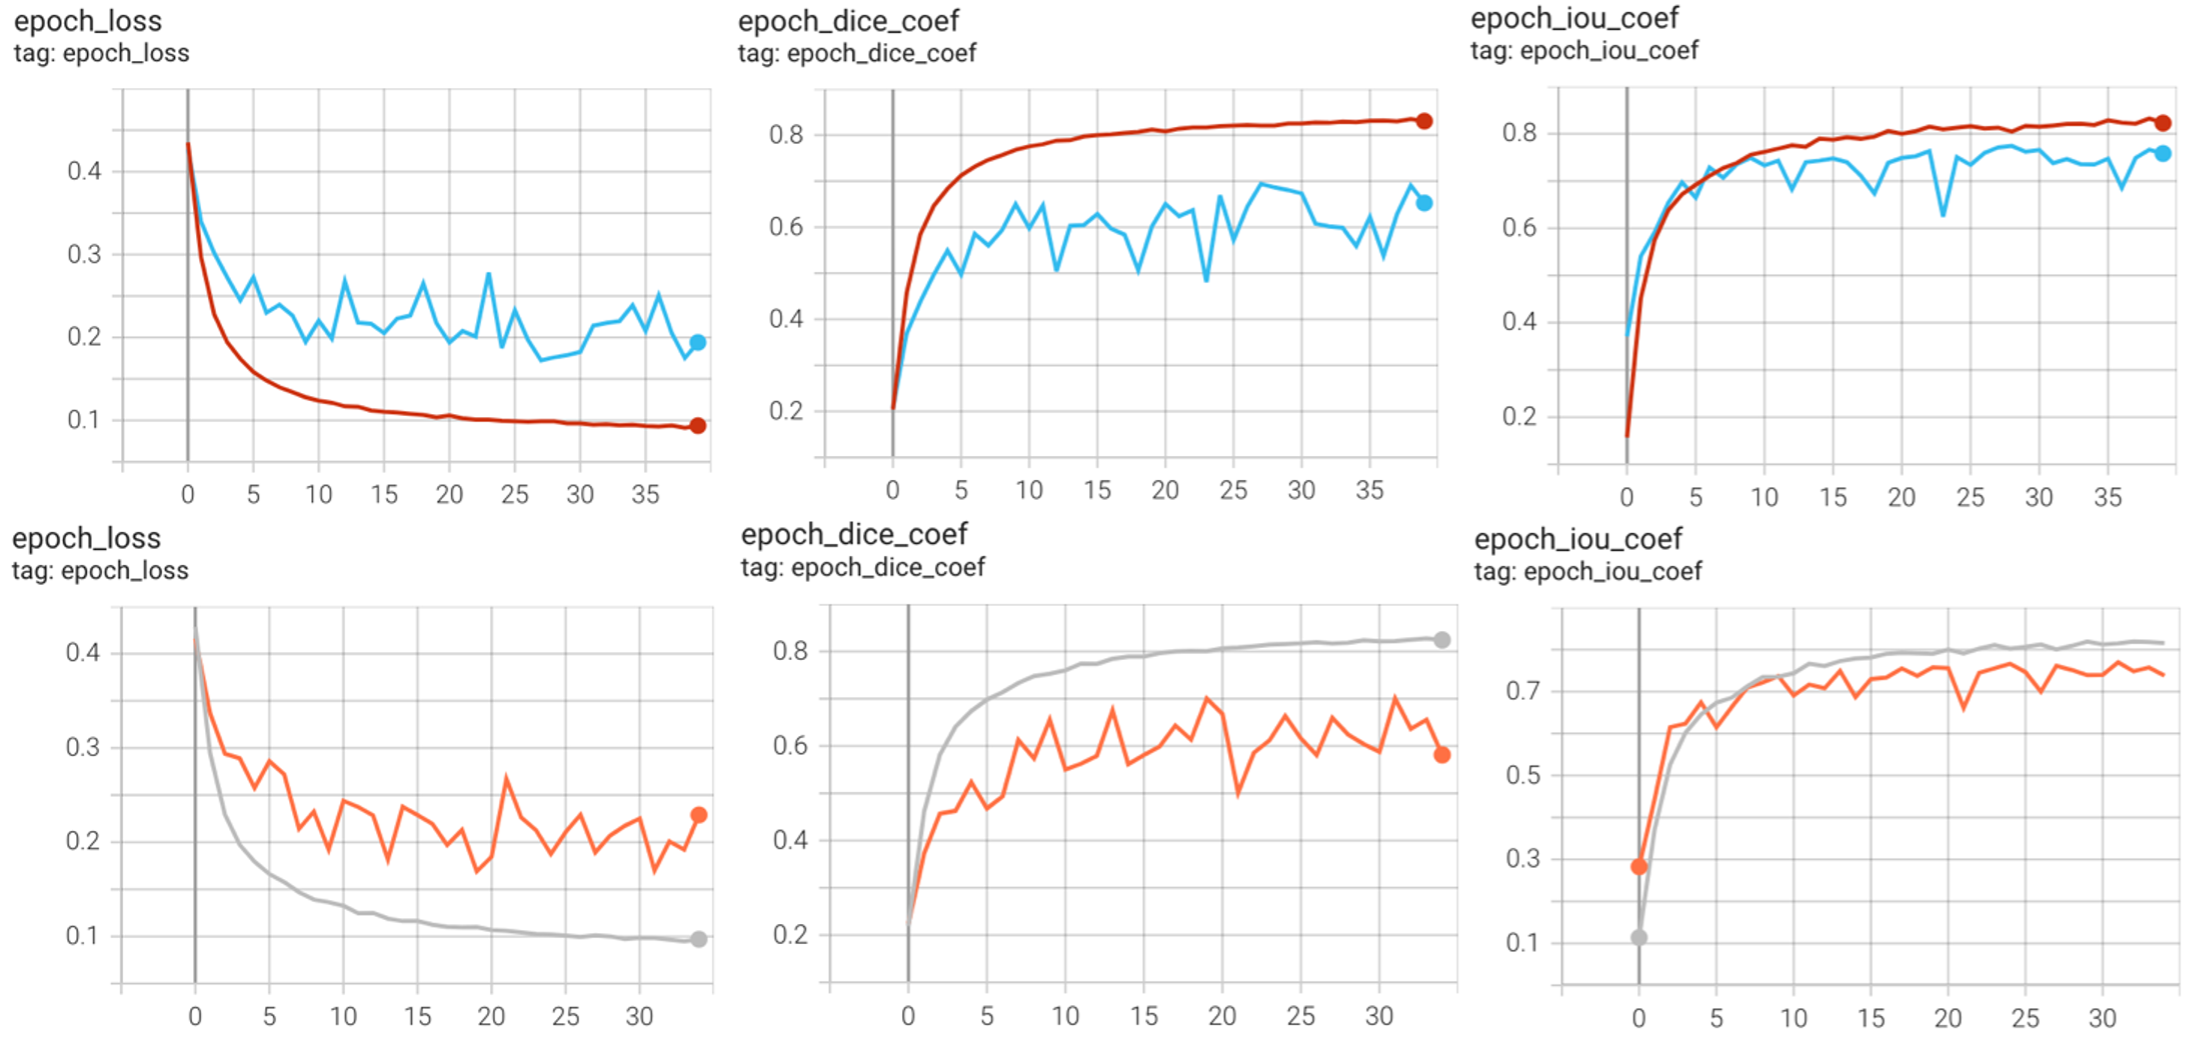
\includegraphics[width = 1\linewidth]{4layers-5layers.png}
  \caption{4层unet和5层unet的损失函数、Dice、IOU优化过程比较;上方:4层unet;下方:5层unet}
  \label{fig:fig10}
\end{figure}

\subsection{不同损失函数的比较}

比较不同的目标损失函数,并对比它们的性能。实验中比较的损失函数有:

\subsubsection{二元交叉熵损失函数}

逐像素的二元交叉熵损失函数有着梯度平滑的优点,但是它的优化易受类别不平衡的影响。定义为:

\[\mathcal{L}_{BCE}(Y,P)=-\frac{1}{N}\sum_{c=1}^{C}\sum_{n=1}^{N}(y_{n,c}\log p_{n,c}+(1-y_{n,c})\log (1-p_{n,c}))\]


\subsubsection{Dice损失函数}

Dice损失函数仅考虑真实掩码和预测掩码的交面积和总面积之比,避免了背景像素占绝大部分比例而导致的类别不平衡问题。但是它有着梯度不平滑的缺点。
\[\mathcal{L}_{Dice}(Y,P)=\sum_{c=1}^{C}(\frac{2Y_{c}P_{c}}{sum(Y_{c})+sum(P_{c})})\]


\subsubsection{soft-dice损失函数}

soft-dice损失函数\cite{c6}考虑在真实类别像素上,对该像素的预测接近1的程度。soft-dice损失函数失去了dice系数的几何意义,它同样能解决类别不平衡问题。
\[\mathcal{L}_{SD}(Y,P)=-\frac{1}{N}\sum_{c=1}^{C}\sum_{n=1}^{N}(\frac{2y_{n,c}p_{n,c}}{y_{n,c}^2+p_{n,c}^2})\]

\subsubsection{二元交叉熵损失函数+Dice损失函数}

合并二元交叉熵损失函数和Dice损失函数,得到混合损失,它既有梯度平滑的优点,也能解决类别不平衡问题。
\[\mathcal{L}_{BCEDice}(Y,P)=\mathcal{L}_{BCE}(Y,P)+\mathcal{L}_{Dice}(Y,P)\]

\subsubsection{二元交叉熵损失函数+Dice损失函数/2}
实验结果表明,二元交叉熵损失函数和0.5的Dice损失函数的混合是较优的组合。
\[\mathcal{L}_{BCEDice_{2:1}}(Y,P)=\mathcal{L}_{BCE}(Y,P)+0.5\times\mathcal{L}_{Dice}(Y,P)\]

表6给出了各损失函数比较的结果。首先,DICE损失函数无法优化,在训练过程中该损失函数不能下降。单独将soft-dice作为损失函数,性能最差,但是平均准确率的结果很好,可能是因为soft-dice损失函数目标隐含了提高平均准确率的目标。单独使用二元交叉熵损失函数的性能不如混合损失函数,原因可能是遭到了类别不平衡的影响。最后,2:1的BCE-DICE损失函数略微优于1:1的BCE-DICE损失函数。然而,混合损失函数的评价准确率在训练过程中均不稳定,这可能是损失函数和平均准确率不相关导致的。

\begin{table}[htbp]
  \centering
  \caption{各损失函数的结果比较;其中轮数表示损失函数极小值所在的最优轮数;DICE、IOU、ACC表示优化过程中的最优值,其下方括号表示该指标在最优轮的数值}
  \label{tab:table6}
  \begin{tabular}{ccccc}
    \toprule
    损失函数&轮数&DICE&IOU&ACC \\
    \midrule
      $BCE$&25&\makecell[c]{0.6786 \\(0.4241)}&\makecell[c]{0.7305 \\ (0.3747)}&\makecell[c]{0.6786 \\ (0.4241)} \\
    \midrule
      $DICE$&/&/&/&/ \\
    \midrule
      $SD$&37&\makecell[c]{0.448\\(0.4458)}&\makecell[c]{0.5678\\(0.5309)}&\makecell[c]{0.9683\\(0.9548)} \\
    \midrule
      $BCEDICE$&36&\makecell[c]{0.6957\\(0.6957)}&\makecell[c]{0.7665\\(0.7631)}&\makecell[c]{0.8628\\(0.1534)} \\
    \midrule
      $BCEDICE_{2:1}$&19&\makecell[c]{0.7006\\(0.7006)}&\makecell[c]{0.7699\\(0.7576)}&\makecell[c]{0.9287\\(0.6449)} \\
    \bottomrule
   \end{tabular}
\end{table}

\begin{figure}[htbp]
  \centering
  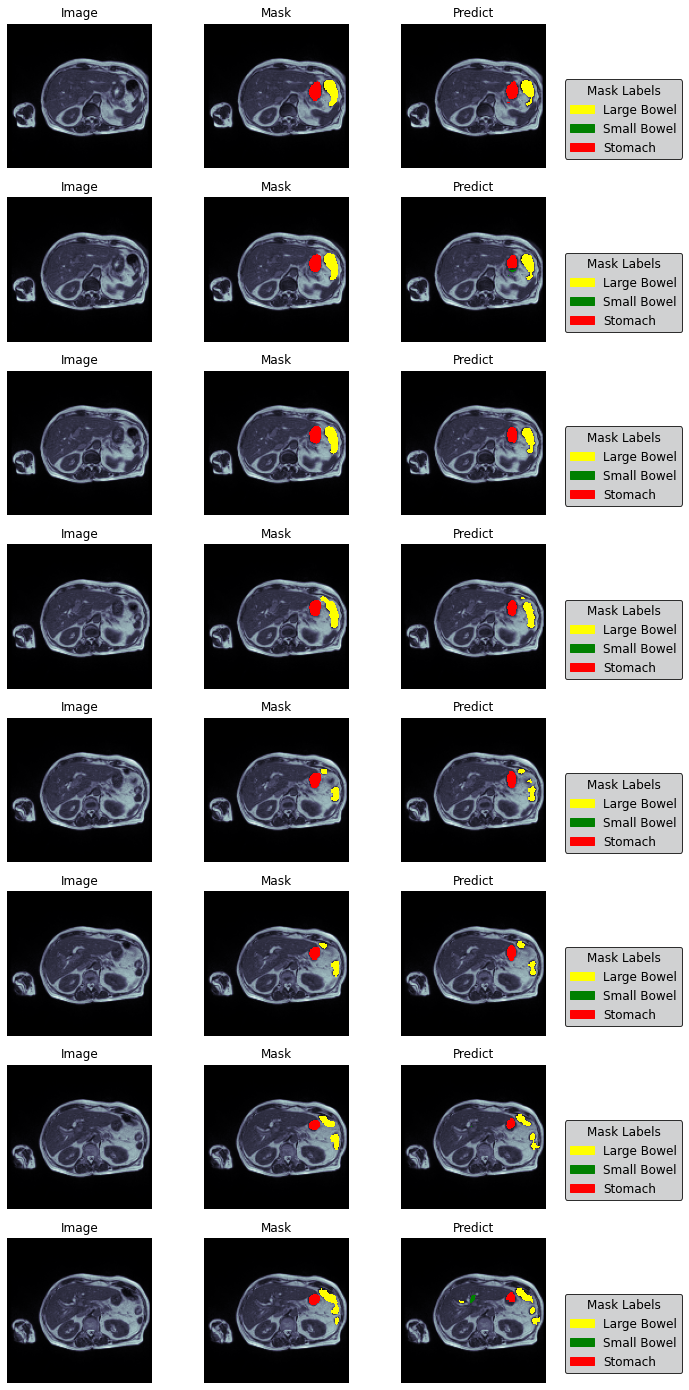
\includegraphics[width = 1\linewidth]{predict_visual.png}
  \caption{原图、真实掩码和预测掩码的可视化}
  \label{fig:fig11}
\end{figure}

\section{结论}

分析了肠胃道图像分割竞赛数据的特点,包括掩码类别的占比、病例扫描次数分布、不同器官类别的共现性。通过观察掩码的重叠,制定了多标签分类的任务类型。分析了在扫描切片维度的掩码分布变化。提出用于胃肠道MRI扫描图像分割的三种改进方法,增加两种注意力机制,在输入张量的特征通道中纳入了邻居扫描图片,修改了U-Net以适用于竞赛数据集,设计了不同参数和下采样深度的两种U-Net变形结构,对比了两种结构的性能,并选择了结构较简单且泛化性能较优的4层U-Net结构。通过应用弹性畸变和高斯模糊,充实了训练数据,极大地提高了U-Net的泛化性能,改善了过拟合的问题。探究了几种损失函数,探究了其可用性,比较了不同损失函数的优缺点,通过实验确定了目前最佳比例的混合损失函数,并分析了平均准确率较低的可能的原因。

目前,仍有以下问题需要解决,并提出相应的改进思路:

第一,在Dice系数和IOU系数提升的同时,平均准确率变得十分不稳定,且在loss最优时准确率较低,在loss非最优时准确率却能达到极大值。说明损失函数和准确率没有相关性。同时,soft-dice损失函数却有着与准确率一致的特点。目前对于背后原因的理论分析不足,对于损失函数或需要更多的改进和取舍。

第二,通过观察模型预测结果,发现除错分类以外,模型还经常漏分类,以及对于正确的分类,预测的掩码的边界相对正确的掩码边界有所收缩,即预测过于保守。然而,对于原始数据的观察发现,有时候模型预测的掩码的收缩反而是正确的,因为专家标注有时过于随意,标注的掩码超出了真实掩码的边界许多。

未来的工作将:改进损失函数,使模型更多关注平均准确率;改进模型,解决预测边界过于保守的问题,或进行数据清洗,解决专家标注过于激进的问题。

\begin{figure}[htbp]
  \centering
  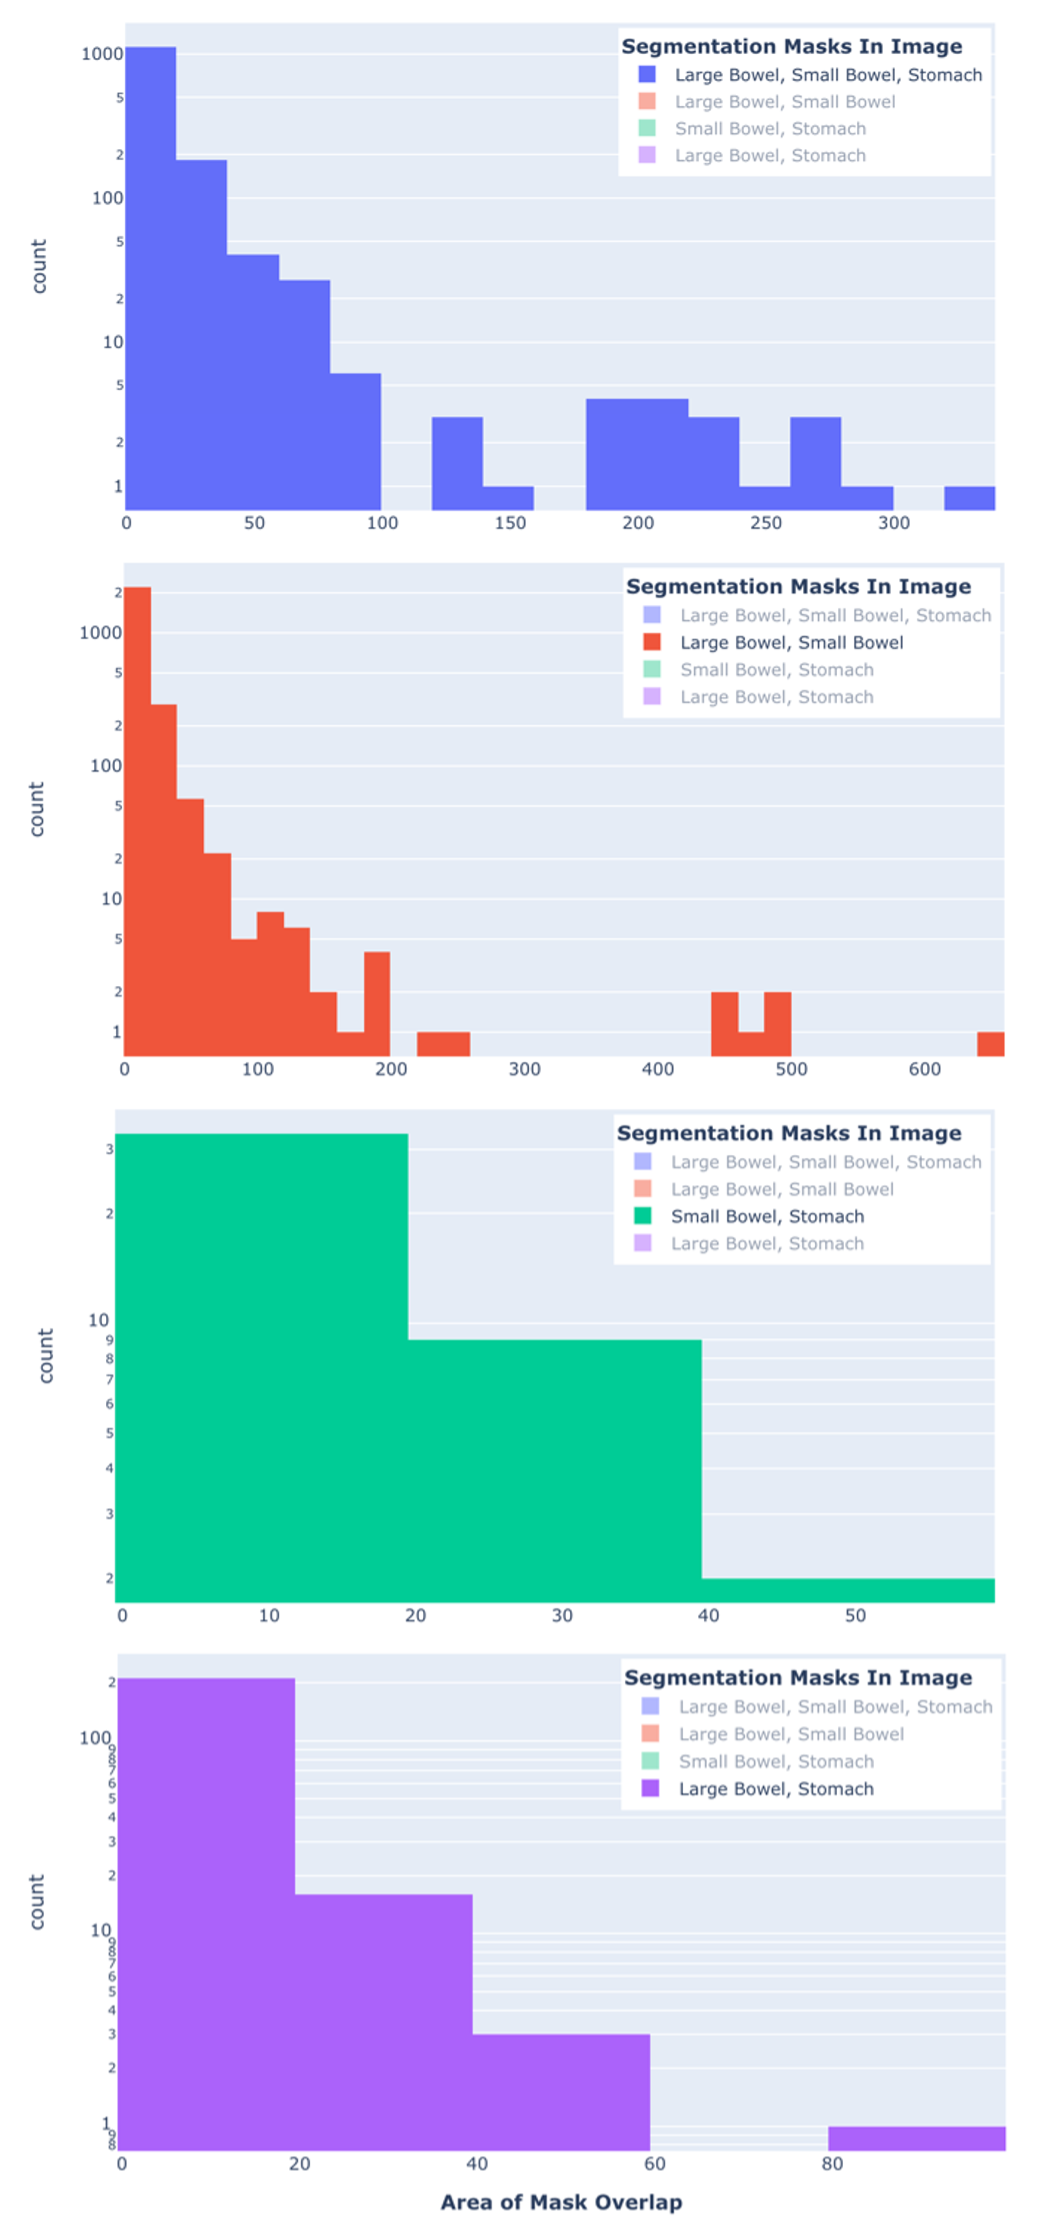
\includegraphics[width = 1\linewidth]{seg_overlay_distribution.png}
  \caption{分割掩码重叠面积的分布}
  \label{fig:fig12}
\end{figure}

\begin{thebibliography}{99}

\bibitem{c1}田娟秀, et al. 医学图像分析深度学习方法研究与挑战. 自动化学报, 2018, 44.3: 401-424.

\bibitem{c2}https://www.kaggle.com/competitions/uw-madison-gi-tract-image-segmentation

\bibitem{attention}VASWANI, Ashish, et al. Attention is all you need. Advances in neural information processing systems, 2017, 30.

\bibitem{MTM}WANG, Hongyi, et al. Mixed transformer u-net for medical image segmentation. In: ICASSP 2022-2022 IEEE International Conference on Acoustics, Speech and Signal Processing (ICASSP). IEEE, 2022. p. 2390-2394.

\bibitem{EA}GUO, Meng-Hao, et al. Beyond self-attention: External attention using two linear layers for visual tasks. arXiv preprint arXiv:2105.02358, 2021.

\bibitem{c3}RONNEBERGER, Olaf; FISCHER, Philipp; BROX, Thomas. U-net: Convolutional networks for biomedical image segmentation. In: International Conference on Medical image computing and computer-assisted intervention. Springer, Cham, 2015. p. 234-241.

\bibitem{c4}LIN, Tsung-Yi, et al. Focal loss for dense object detection. In: Proceedings of the IEEE international conference on computer vision. 2017. p. 2980-2988.

\bibitem{c5}P. Y. Simard, D. Steinkraus and J. C. Platt, "Best practices for convolutional neural networks applied to visual document analysis," Seventh International Conference on Document Analysis and Recognition, 2003. Proceedings., 2003, pp. 958-963, doi: 10.1109/ICDAR.2003.1227801.

\bibitem{c6}Z. Zhou, M. M. R. Siddiquee, N. Tajbakhsh and J. Liang, "UNet++: Redesigning Skip Connections to Exploit Multiscale Features in Image Segmentation," in IEEE Transactions on Medical Imaging, vol. 39, no. 6, pp. 1856-1867, June 2020, doi: 10.1109/TMI.2019.2959609.


\end{thebibliography}
\end{document}
